\section{Créer un dépôt}

Contrairement à \acl{svn}, Git fonctionne à la fois en local et sur le serveur : chaque client contient son propre dépôt local.\\
Le dépôt en ligne ne permet que de synchroniser les différents dépôts locaux.\\

Pour commencer, nous allons travailler \textbf{hors-ligne} :

\subsection*{Par ligne de commande}
\begin{verbatim}
# Creer un dossier "test" et s'y rend
$ mkdir ~/test
$ cd ~/test

# Crée un dépôt dans le dossier courant
$ git init
\end{verbatim}

Voilà. C'est tout. Un dossier ".git" doit être apparu.
Sous git bash (sous windows) vous devriez voir une invite de commande indiquant la branche sur laquelle vous êtes (master).

Pour savoir si votre dépôt est actif, tapez :
\begin{verbatim}
$ git status

# En cas d'erreur :
fatal: Not a git repository (or any of the parent directories): .git

# En cas de réussite :
# On branch master
nothing to commit, working directory clean
\end{verbatim}

\subsection*{Par tortoise git}
Creez un nouveau dossier $\rightarrow$ Clic droit dessus $\rightarrow$ Create git repository here

Voilà. C'est tout. Un dossier ".git" doit être apparu.

Pour savoir si votre dépôt est actif, faites un clic droit : les options de tortoise git ont du changer.
Vous devirez pouvoir faire des commit, push, fetch, etc..

\begin{figure}[h] 
	\begin{center}
		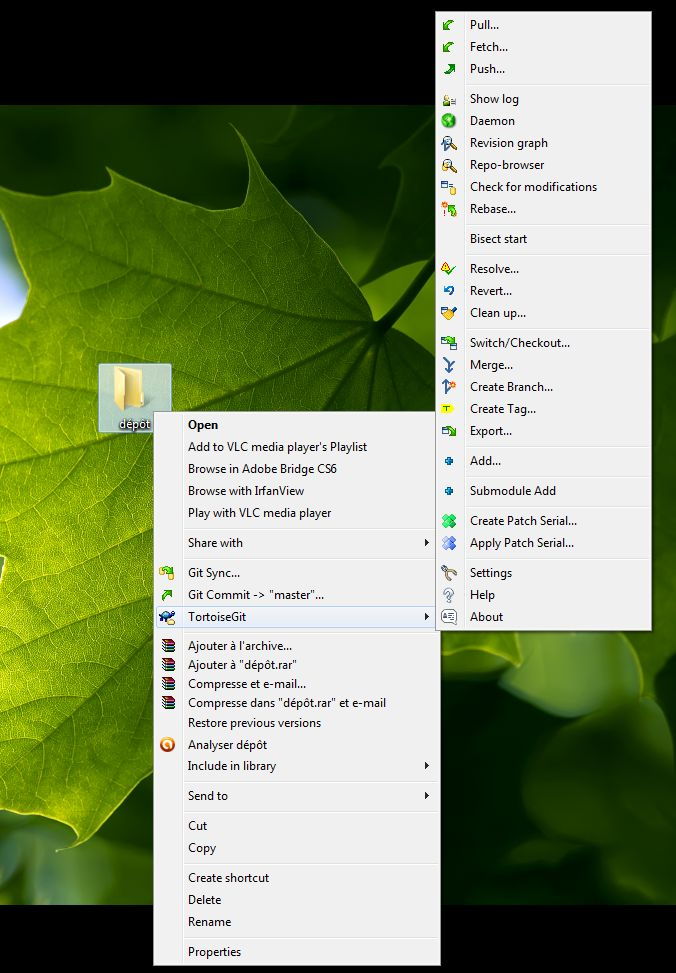
\includegraphics[scale=0.2]{../IMG/menuTG.jpg}
	\end{center}
	\caption{Tortoise Git : Le menu du depot}
	\label{Tortoise Git : Le menu du depot} 
\end{figure}